% ===========================================================
% CAPA CUSTOMIZADA INSPER
% Input este arquivo no preamble: % ===========================================================
% CAPA CUSTOMIZADA INSPER
% Input este arquivo no preamble: % ===========================================================
% CAPA CUSTOMIZADA INSPER
% Input este arquivo no preamble: % ===========================================================
% CAPA CUSTOMIZADA INSPER
% Input este arquivo no preamble: \input{capa_insper}
% ===========================================================

\usepackage{tikz}
\usetikzlibrary{calc}
\usepackage{geometry}

\renewcommand{\imprimircapa}{%
  \begin{capa}%
    \newgeometry{left=25mm,right=25mm,top=25mm,bottom=25mm}%
    \thispagestyle{empty}%

    % ------ Topo: logo e curso ------
    \begin{center}
      
\includegraphics[width=40mm]{insper-logo}%
    \end{center}

    \vspace{4mm}
    \begin{center}
      {\small\imprimircurso}
    \end{center}

    % ------ Blocos com imagens PNG ------
    \begin{tikzpicture}[remember picture, overlay]

      \coordinate (cc) at ($(current page.center)+(0,0.9cm)$);

      \def\BW{12.8cm}
      \def\BH{5.8cm}
      \def\PAD{0.9cm}
      \def\GW{13.2cm}
      \def\GH{5.6cm}
      \def\RW{13.2cm}
      \def\RH{5.4cm}

      % Fundo Cinza
      \node[anchor=center, inner sep=0pt]
        at ($(cc)+(-1.1cm,0.6cm)$)
        {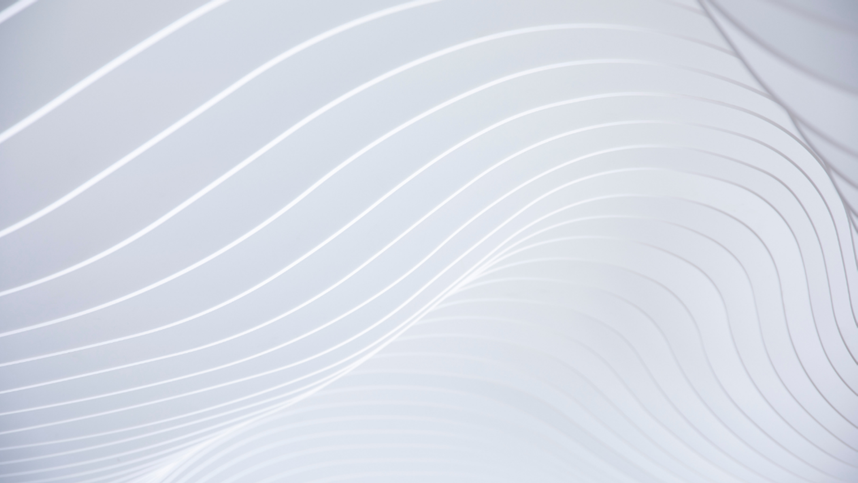
\includegraphics[width=\GW, height=\GH,
          keepaspectratio=false]{FundoCinza}};

      % Fundo Vermelho
      \node[anchor=center, inner sep=0pt]
        at ($(cc)+(1.0cm,-0.7cm)$)
        {
\includegraphics[width=\RW, height=\RH,
          keepaspectratio=false]{FundoVermelho}};

      % Fundo Preto (âncora para título e autor)
      \node[inner sep=0pt, minimum width=\BW, minimum height=\BH,
            anchor=center] (blk) at (cc)
        {
\includegraphics[width=\BW, height=\BH,
          keepaspectratio=false]{FundoPreto}};

      % Título
      \node[anchor=north west, text=white, align=left, text width=11.1cm]
        at ($(blk.north west)+(\PAD,-\PAD)$)
        {\bfseries\fontsize{22pt}{26pt}\selectfont \imprimirtitulo};

      % Autor
      \node[anchor=south west, text=white]
        at ($(blk.south west)+(\PAD,\PAD)$)
        {\large\bfseries \imprimirautor};

    \end{tikzpicture}

    % ------ Rodapé ------
    \vfill
    \begin{center}
      \imprimirlocal\\
      \imprimirdata
    \end{center}

    \restoregeometry
  \end{capa}%
}
% ===========================================================

\usepackage{tikz}
\usetikzlibrary{calc}
\usepackage{geometry}

\renewcommand{\imprimircapa}{%
  \begin{capa}%
    \newgeometry{left=25mm,right=25mm,top=25mm,bottom=25mm}%
    \thispagestyle{empty}%

    % ------ Topo: logo e curso ------
    \begin{center}
      
\includegraphics[width=40mm]{insper-logo}%
    \end{center}

    \vspace{4mm}
    \begin{center}
      {\small\imprimircurso}
    \end{center}

    % ------ Blocos com imagens PNG ------
    \begin{tikzpicture}[remember picture, overlay]

      \coordinate (cc) at ($(current page.center)+(0,0.9cm)$);

      \def\BW{12.8cm}
      \def\BH{5.8cm}
      \def\PAD{0.9cm}
      \def\GW{13.2cm}
      \def\GH{5.6cm}
      \def\RW{13.2cm}
      \def\RH{5.4cm}

      % Fundo Cinza
      \node[anchor=center, inner sep=0pt]
        at ($(cc)+(-1.1cm,0.6cm)$)
        {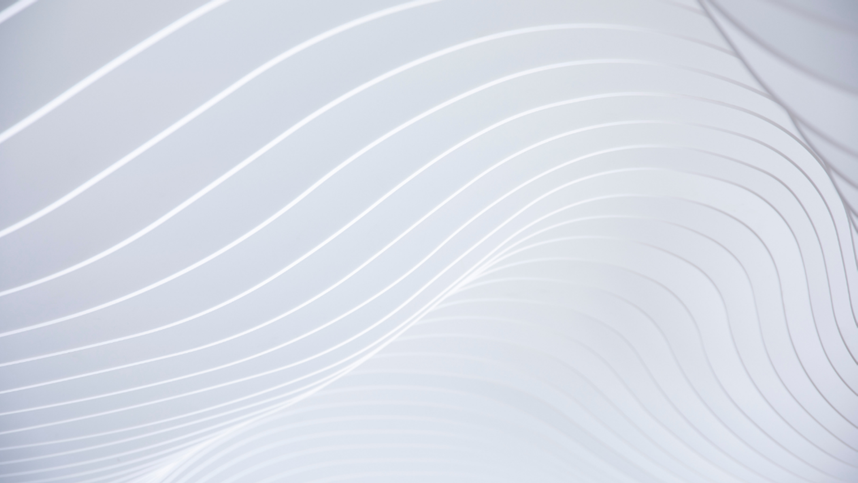
\includegraphics[width=\GW, height=\GH,
          keepaspectratio=false]{FundoCinza}};

      % Fundo Vermelho
      \node[anchor=center, inner sep=0pt]
        at ($(cc)+(1.0cm,-0.7cm)$)
        {
\includegraphics[width=\RW, height=\RH,
          keepaspectratio=false]{FundoVermelho}};

      % Fundo Preto (âncora para título e autor)
      \node[inner sep=0pt, minimum width=\BW, minimum height=\BH,
            anchor=center] (blk) at (cc)
        {
\includegraphics[width=\BW, height=\BH,
          keepaspectratio=false]{FundoPreto}};

      % Título
      \node[anchor=north west, text=white, align=left, text width=11.1cm]
        at ($(blk.north west)+(\PAD,-\PAD)$)
        {\bfseries\fontsize{22pt}{26pt}\selectfont \imprimirtitulo};

      % Autor
      \node[anchor=south west, text=white]
        at ($(blk.south west)+(\PAD,\PAD)$)
        {\large\bfseries \imprimirautor};

    \end{tikzpicture}

    % ------ Rodapé ------
    \vfill
    \begin{center}
      \imprimirlocal\\
      \imprimirdata
    \end{center}

    \restoregeometry
  \end{capa}%
}
% ===========================================================

\usepackage{tikz}
\usetikzlibrary{calc}
\usepackage{geometry}

\renewcommand{\imprimircapa}{%
  \begin{capa}%
    \newgeometry{left=25mm,right=25mm,top=25mm,bottom=25mm}%
    \thispagestyle{empty}%

    % ------ Topo: logo e curso ------
    \begin{center}
      
\includegraphics[width=40mm]{insper-logo}%
    \end{center}

    \vspace{4mm}
    \begin{center}
      {\small\imprimircurso}
    \end{center}

    % ------ Blocos com imagens PNG ------
    \begin{tikzpicture}[remember picture, overlay]

      \coordinate (cc) at ($(current page.center)+(0,0.9cm)$);

      \def\BW{12.8cm}
      \def\BH{5.8cm}
      \def\PAD{0.9cm}
      \def\GW{13.2cm}
      \def\GH{5.6cm}
      \def\RW{13.2cm}
      \def\RH{5.4cm}

      % Fundo Cinza
      \node[anchor=center, inner sep=0pt]
        at ($(cc)+(-1.1cm,0.6cm)$)
        {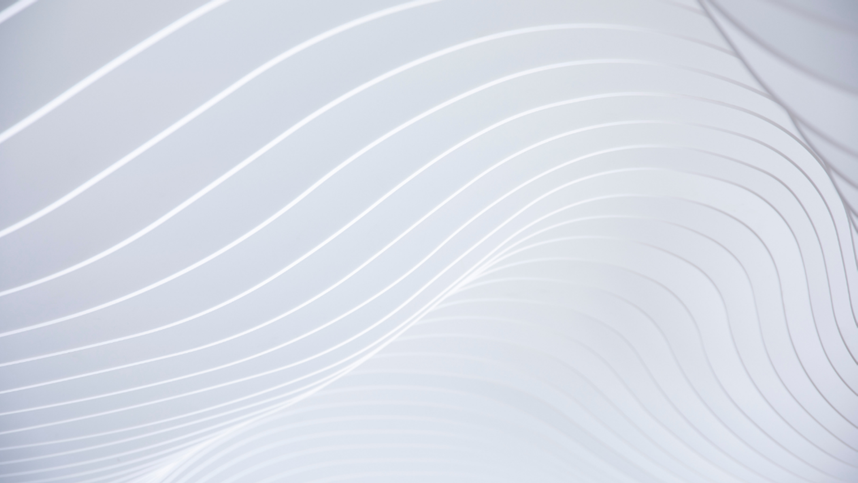
\includegraphics[width=\GW, height=\GH,
          keepaspectratio=false]{FundoCinza}};

      % Fundo Vermelho
      \node[anchor=center, inner sep=0pt]
        at ($(cc)+(1.0cm,-0.7cm)$)
        {
\includegraphics[width=\RW, height=\RH,
          keepaspectratio=false]{FundoVermelho}};

      % Fundo Preto (âncora para título e autor)
      \node[inner sep=0pt, minimum width=\BW, minimum height=\BH,
            anchor=center] (blk) at (cc)
        {
\includegraphics[width=\BW, height=\BH,
          keepaspectratio=false]{FundoPreto}};

      % Título
      \node[anchor=north west, text=white, align=left, text width=11.1cm]
        at ($(blk.north west)+(\PAD,-\PAD)$)
        {\bfseries\fontsize{22pt}{26pt}\selectfont \imprimirtitulo};

      % Autor
      \node[anchor=south west, text=white]
        at ($(blk.south west)+(\PAD,\PAD)$)
        {\large\bfseries \imprimirautor};

    \end{tikzpicture}

    % ------ Rodapé ------
    \vfill
    \begin{center}
      \imprimirlocal\\
      \imprimirdata
    \end{center}

    \restoregeometry
  \end{capa}%
}
% ===========================================================

\usepackage{tikz}
\usetikzlibrary{calc}
\usepackage{geometry}

\renewcommand{\imprimircapa}{%
  \begin{capa}%
    \newgeometry{left=25mm,right=25mm,top=25mm,bottom=25mm}%
    \thispagestyle{empty}%

    % ------ Topo: logo e curso ------
    \begin{center}
      
\includegraphics[width=40mm]{insper-logo}%
    \end{center}

    \vspace{4mm}
    \begin{center}
      {\small\imprimircurso}
    \end{center}

    % ------ Blocos com imagens PNG ------
    \begin{tikzpicture}[remember picture, overlay]

      \coordinate (cc) at ($(current page.center)+(0,0.9cm)$);

      \def\BW{12.8cm}
      \def\BH{5.8cm}
      \def\PAD{0.9cm}
      \def\GW{13.2cm}
      \def\GH{5.6cm}
      \def\RW{13.2cm}
      \def\RH{5.4cm}

      % Fundo Cinza
      \node[anchor=center, inner sep=0pt]
        at ($(cc)+(-1.1cm,0.6cm)$)
        {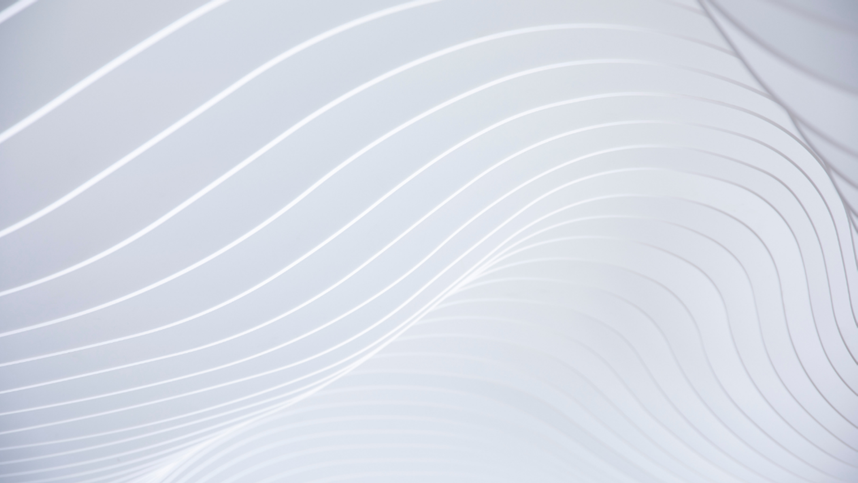
\includegraphics[width=\GW, height=\GH,
          keepaspectratio=false]{FundoCinza}};

      % Fundo Vermelho
      \node[anchor=center, inner sep=0pt]
        at ($(cc)+(1.0cm,-0.7cm)$)
        {
\includegraphics[width=\RW, height=\RH,
          keepaspectratio=false]{FundoVermelho}};

      % Fundo Preto (âncora para título e autor)
      \node[inner sep=0pt, minimum width=\BW, minimum height=\BH,
            anchor=center] (blk) at (cc)
        {
\includegraphics[width=\BW, height=\BH,
          keepaspectratio=false]{FundoPreto}};

      % Título
      \node[anchor=north west, text=white, align=left, text width=11.1cm]
        at ($(blk.north west)+(\PAD,-\PAD)$)
        {\bfseries\fontsize{22pt}{26pt}\selectfont \imprimirtitulo};

      % Autor
      \node[anchor=south west, text=white]
        at ($(blk.south west)+(\PAD,\PAD)$)
        {\large\bfseries \imprimirautor};

    \end{tikzpicture}

    % ------ Rodapé ------
    \vfill
    \begin{center}
      \imprimirlocal\\
      \imprimirdata
    \end{center}

    \restoregeometry
  \end{capa}%
}